\section{Example}
\begin{figure}[h]
	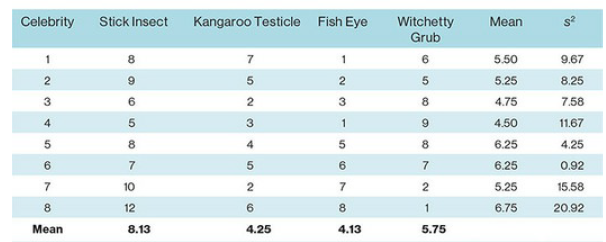
\includegraphics[width=1\textwidth,height=60mm]{Chapter 15 GLM 4 Repeated-measures designs/example.PNG}
	\caption{Sample size of 8, each participant goes through 4 different conditions. }
\end{figure}

For this the equation is:
\begin{equation}
\begin{split}
\text{Retch}_{gi} & = b_{0i} + b_{1i}X_{gi} + \varepsilon_{gi} \\
b_{0i} & = b_0 + u_{0i}\\
b_{1i} & = b_0 + u_{1i}
\end{split}
\end{equation}

Subscript $i$ is used to denote each individual. And the different predictors is denoted by $g$. So we can predict retch time ($Y_{gi}$) for food $g$ within person $i$  from the specific food eaten ($X_{gi}$).

However, we need to factor in that individuals will vary in their constitution. We can do this by adding a variance term to the intercept. Intercept represents time to wretch when predictor is 0; so if we allow this parameter $b_{0i}$ to vary across individuals, we are effectively modelling the possibility that different people will have different retching latency. We define $b_{0i}$ as made up of the group level intercept ($b_0$) plus the deviation of the individual's intercept from the group-level intercept ($u_{0i}$). So $u_{0i}$ is the individual differences in retching. 

Similarly, for the slope, we also have to account for individual's deviation of the group slope. So for $b_1$, we also split the variables into $b_1$ and $u_{1i}$. $u_i$ reflects individual's differences in the effect of food on retching.

First line of equation (7.1) models the individual. Second and third line models the group level effects.

So we assume that the variation within conditions is similar and that no two conditions are any more dependent than any other two.

\section{Assumption of sphericity}
\textbf{Sphericity} is about assuming that the relationship between scores in pairs of treatment conditions is similar (i.e. level of dependence between means is roughly equal).

The assumption of sphericity (denoted by $\varepsilon$ and sometimes referred to as circularity) can be likened to the assumption of homogeneity of variance in between-group designs. It is a form of compound symmetry, which holds true when both the variances across conditions are equal. and the covariances between pairs of conditions are equal.

Sphericity is a more general, less restrictive form of compound symmetry and refers to the equality of variances of the differences between treatment levels

\begin{figure}[h]
	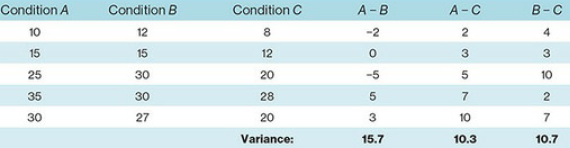
\includegraphics[width=1\textwidth,height=50mm]{Chapter 15 GLM 4 Repeated-measures designs/sphericity.PNG}
	\caption{3 different conditions and differences of each conditions }
\end{figure}

Sphericity will hold when:
\begin{center}
$\text{variance}_{A-B} \approx \text{variance}_{A-C} \approx \text{variance}_{B-C} $
\end{center}

In this example, there is some deviation from sphericity in the data as variance of A-B is greater than the rest. However, the data has local circularity (local sphericity) as two of the variances of differences are very similar, which means that sphericity can be assumed for any multiple comparisons involving these conditions.

But how do we know whether the difference in variance of differences is large enough to be a problem?

\section{Assessing the severity of departures from sphericity}
We can use Mauchly's test to assess the hypothesis that the variances of the differences between conditions are equal. If Mauchly's test statistic is significant, it implies that there are significant differences between the variances of differences and,therefore, sphericity is not met.  If Mauchly's test is non significant ($p > .05$), then it means variances of differences are roughly equal and sphericity is met.

Downside of Mauchly test is that it is a significance test so it depends on sample size. So in large sample size, Mauchly test could mean just a small departure from sphericity that we have a lot of power to detect, and in small sample size, Mauchly test can mean a large departure from sphericity but we do not have power to detect. So either ways we always just use the Greenhouse-Geisser correction

Instead, we can estimate the degree of sphericity using Greenhouse-Geisser estimate $\hat{\varepsilon}$. 

The degree to which sphericity is present, or not, is represented by a statistic called epsilon ($\hat{\varepsilon}$). An epsilon of 1 (i.e., $\hat{\varepsilon} = 1$) indicates that the condition of sphericity is exactly met. The further epsilon decreases below 1 (i.e., $\hat{\varepsilon}< 1$), the greater the violation of sphericity. Therefore, you can think of epsilon as a statistic that describes the degree to which sphericity has been violated. The lowest value that  $\hat{\varepsilon}$ can take is called the lower-bound estimate, upper limit is 1. 

Greenhouse-Geisser estimate varies between 1/(k-1) and 1, where k is the number of repeated conditions. e.g. if there are 5 conditions, the lower limit of $\hat{\varepsilon}$ is 1/(5-1) = 0.25, and upper limit is 1.

\section{Effect of violating the assumption of sphericity}
Sphericity creates a loss of power and an F-statistic that does not have the distribution that it's supposed to have (i.e. an F-distribution).

Lack of sphericity causes some complications for post hoc tests. If you dont want to worry about what these complications are when sphericity is violated, then the Bonferroni method is the most robust in terms of power and control of Type I error rate.

When sphericity is not violated, Tukey's test can be used.

\textbf{Note:} sphericity is not relevant if you are comparing only two means. The assumption is that the variances of difference scores between pairs of treatment levels are equal, and with only two conditions, you have only one set of difference scores and so only 1 variance. You need at least 3 conditions for sphericity to be an issue. 

% Read jane the superbrain 15.1 when you finished between subject ANOVA.

\section{What to do if you violate sphericity?}
If you violate sphericity, just adjust the degrees of freedom of any F-statistics affected. You multiply the degrees of freedom for an affected F by this estimate of sphericity. The result is that when you have sphericity, the degrees of freedom don't change as you are multiplying by 1. But if you dont have sphericity, your degrees of freedom will be smaller (as you are multiplying by less than 1).

Greater violation of sphericity, smaller the estimate, smaller the degrees of freedom.
Smaller df make the p value associated with F-statistic less significant. By adjusting degrees of freedom, we make F-statistics more conservative, and so Type I error is controlled.

\section{F statistics for repeated measures designs}
In repeated measures design, the effect of the experiment (Independent variable) is shown up in within participant variance (rather than in the between-group variance).

In between subject design, the within participant variance is the residual sum of squares ($SS_R$); variance is created by individual differences in performance.

However for repeated measures design, experimental manipulation is carried on the same entities, within participant variance will be made up of not just individual differences in the performance but also effect of the manipulation.


\begin{figure}[t!]
	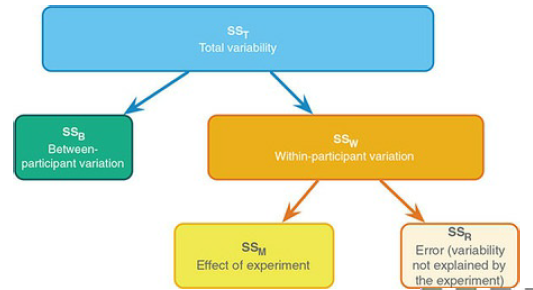
\includegraphics[width=1\textwidth,height=80mm]{Chapter 15 GLM 4 Repeated-measures designs/withinparticipantvariance.PNG}
	\caption{$SS_M$ and $SS_R$ both comes from within participant variation in repeated measures design}
\end{figure}

\section{Total sum of squares, $SS_T$}
Similar to one way independent design, $SS_T$ is calculated as:
\begin{equation}
\text{SS}_T = s^2_{grand}(N-1)
\end{equation}
$df$ for $SS_T$ is also N - 1

\section{Within participant sum of squares,$SS_W$}
For $SS_R$ in a repeated measures design, the most crucial difference is that there is a within participant variance component, which represents individual differences within participants.

 In independent design, there are different participants within each condition, we calculated $SS_R$ within each condition and added these to get a total value.These individual differences were quantified with residual sum of squares ($SS_R$) using the equation:
\begin{equation}
\begin{split}
&\textbf{For independent design}: \\
SS_R& = \sum^k_{g=1} \sum^n_{i=1} (x_{ig}-\bar{x}_g)^2 \\
& = \sum^k_{g=1} s^2_g(n_g - 1)\\
& = s^2_{group1}(n_1 - 1) +  s^2_{group2}(n_2 - 1) + ... +  s^2_{group n}(n_n - 1)
\end{split}
\end{equation}

However, in repeated measures design, we subjected entities to more than one experimental condition, we are interested in the variation not within a condition but \emph{within an entity}. We can adapt similar equation to look within participants rather than groups. We will call this equation $SS_W$ (for within participant SS).

\begin{equation}
\begin{split}
&\textbf{For repeated measures design}: \\
SS_W &= s^2_{entity1}(n_1 - 1) +  s^2_{entity2}(n_2 - 1) + ... +  s^2_{entity n}(n_n - 1)
\end{split}
\end{equation}

In our celebrity example it will be: 
\begin{equation*}
\begin{split}
SS_W & = 9.67(4-1) + 8.25(4-1) + 7.58(4-1) + 11.67(4-1) + 4.25(4-1) + 0.92(4-1) + \\
& 15.58(4-1) + 20.92(4-1) \\
& = 236.50
\end{split}
\end{equation*}
$df$ for each entity is n-1 (i.e. number of conditions minus 1). Total $df$ is just the sum of df of each participants. e.g. 8 participants with 3 df each, there will be 24 df in total. 

\section{Model sum of squares, $SS_M$}
Note that $SS_M$ for within participant design is part of $SS_W$. For independent design, we worked out how much variation could be explained by our experiment (model SS) by looking at the means for each group and comparing these to the overall mean. We do the same in repeated measures design:

\begin{equation}
\text{SS}_M = \sum^k_{g=1} n_g(\bar{x}_g - \bar{x}_{grand})^2
\end{equation}
$\bar{x}_g$ is the group mean of each condition, $\bar{x}_{grand}$ is the grand mean of all condition. $n_g$ is the number of participants in each condition.

In our example, $SS_M$ is:
\begin{equation*}
\begin{split}
SS_M & = 8(8.13-5.56)^2 + 8(4.25-5.56)^2 + 8(4.13-5.56)^2 + 8(5.75-5.56)^2\\
& = 83.13
\end{split}
\end{equation*}

df for $SS_M$ is the number of conditions (k) - 1 (similar to independent design).

\section{Residual sum of squares, $SS_R$}

simplest way is to subtract $SS_M$ from $SS_W$. 
\begin{equation}
SS_R = SS_W - SS_M
\end{equation}

In our example, $SS_R$ = 236.50 - 83.13 = 153.37
similarly df for $SS_R$ is calculated in similar way:
\begin{equation}
df_R = df_W - df_M
\end{equation}
In our example, df is 24-3= 21. 

\section{Mean Squares and F-statistics}

\begin{equation}
\begin{split}
MS_M & = \frac{SS_M}{df_M} \\
MS_R & = \frac{SS_R}{df_R} \\
\end{split}
\end{equation}

\begin{equation}
F = \frac{MS_M}{MS_R}
\end{equation}

In our example: $MS_M = \frac{83.13}{3} = 27.71, MS_R = \frac{153.37}{21} = 7.30$

$F = \frac{27.71}{7.30} = 3.79$

\section{Between Participant sum of squares, $SS_B$}
Just need to subtract within participant sum of squares with total sum of squares
\begin{equation}
SS_B = SS_T - SS_W
\end{equation}